Anyone using a word processing tool such as Microsoft Word has come across a spell checking component that indicates spelling mistakes and proposes corrections. 40 years after the first spelling correction program by Ralph Gorin, language checkers nowadays do not simply compare the list of extracted words against a dictionary of correctly spelled words, but have become increasingly sophisticated. In addition to language-dependent algorithms for handling \underbar{morphology} (e.g. plural formation), some are now capable of recognizing syntax–related errors, such as a missing verb or a verb that does not agree with its subject in person and number, e.g. in ‘She *\emph{write} a letter.’ However, most available spell checkers (including Microsoft Word) will find no errors in the following first verse of a poem by Jerrold H. Zar (1992)\footnote{\url{http://www.bios.niu.edu/zar/zar.shtml}}: 

\begin{verse}
\emph{%
Eye have a spelling chequer,\\
It came with my Pea Sea.\\
It plane lee marks four my revue\\
Miss Steaks I can knot sea.
}
\end{verse}

For handling these types of errors, analysis of the context is needed in many cases, e.g., for deciding if a word needs to be written with “y” or “i”, as in:

\begin{verse}
\emph{%
Kto chce psa biť, palicu si nájde.\\
{[}He who wants to beat a dog will find a stick.{]}\\
\smallskip
Kto chce psom byť, pána si nájde.\\
{[}He who wants to be a dog will find his master.{]}
}
\end{verse}

This either requires the formulation of language-specific \underbar{grammar} rules, i.e. a high degree of expertise and manual labour, or the use of a so-called statistical \underbar{language model}.  Such models calculate the probability of a particular word occurring in a specific environment (i.e., the preceding and following words). For example, \emph{chce psom byť} is a much more probable word sequence than \emph{chce psom biť}, and \emph{chce psa biť} is a much more probable sentence than \emph{chce psa byť} (nevertheless, we can contrive contexts where all four sequences are grammatical). A statistical language model can be automatically derived using a large amount of (correct) language data (i.e. a \underbar{corpus}). Up to now, these approaches have mostly been developed and evaluated on English language data. However, they do not necessarily transfer straightforwardly to Slovak with its flexible word order and richer inflection. 

\begin{figure*}[htb]
  \colorrule{grey3}{\textwidth}{1.5pt}
  \center
  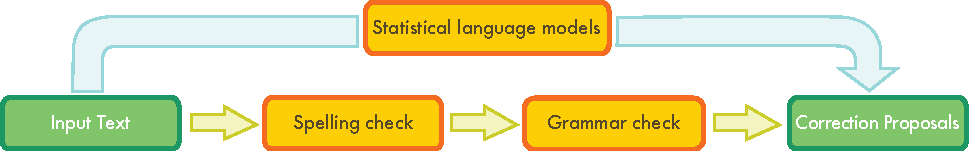
\includegraphics[width=\textwidth]{../_media/english/language_checking}
  \caption{Language checking (statistical; rule-based)}
  \label{fig:langcheckingaarch_en}
  \colorrule{grey3}{\textwidth}{1.5pt}
\end{figure*}

The use of Language Checking is not limited to word processing tools, but is also applied in authoring support systems. Accompanying the rising number of technical products, the amount of technical documentation has rapidly increased over the last decades. Fearing customer complaints about wrong usage and damage claims resulting from bad or badly understood instructions, companies have begun to increasingly focus on the quality of technical documentation, at the same time targeting the international market. Advances in NLP lead to the development of authoring support software, which assists the writer of technical documentation to use vocabulary and sentence structures consistent with certain rules and terminology restrictions.

\boxtext{The spelling checkers for Slovak are mostly based on a dictionary of basic word forms (lemmas)}

The existing spelling checkers for Slovak are mostly based on a dictionary of basic word forms (lemmas) combined with a set of morphological rules enabling the analysis or generation of all (correct) word forms. Although this simple approach seems to be satisfactory, it has two substantial drawbacks. The first issue concerns the superficially correct word forms appearing in a wrong context. The second drawback is the inability to distinguish between real spelling errors and word forms which are correct, but which are not contained in the dictionary. Such words will always exist due to the natural enhancement of a lexicon by newly created words, by new scientific or technical terms etc.

Besides spell checkers and authoring support, Language Checking is also important in the field of computer-assisted language learning. Language checking applications also automatically correct search engine queries, e.g. Google’s ‘Did you mean\dots’ suggestions. 
